% chapter03.tex

 %%%%%%%%%%%%%%%%%%%%%%%%%%%%%%%%%%%%%%%%%%%%%%%%%%%%%%%%%%%%%%%%%%%%%%%%%%%%%
 %                                                                           %
 %    PyMS documentation                                                     %
 %    Copyright (C) 2005-8 Vladimir Likic                                    %
 %                                                                           %
 %    The files in this directory provided under the Creative Commons        %
 %    Attribution-NonCommercial-NoDerivs 2.1 Australia license               %
 %    http://creativecommons.org/licenses/by-nc-nd/2.1/au/                   %
 %    See the file license.txt                                               %
 %                                                                           %
 %%%%%%%%%%%%%%%%%%%%%%%%%%%%%%%%%%%%%%%%%%%%%%%%%%%%%%%%%%%%%%%%%%%%%%%%%%%%%

\chapter{Data pre-processing}

\section{Noise smoothing in ion chromatograms}

\noindent
[ {\em This example is in pyms-test/11} ]

Noise smoothing is usually the first step in raw data pre-processing. The
purpose of noise smoothing is to remove high-frequency noise from data, and
thereby increase the contribution of the signal relative to the contribution
of the noise.

One simple approach to noise smoothing is moving average window smoothing.
In this approach a window of fixed size $2N+1$ points is moved across the ion
chromatogram, and the value at each point is replaced with the mean intensity
over the window size. The pyms-test/11/ illustrates this. The script proc.py
is given below:

\begin{verbatim}
01  """proc.py
02  """
03  
04  import sys
05  sys.path.append("/home/current/proj/PyMS/")
06  
07  from pyms.IO.ANDI.Class import ChemStation
08  from pyms.Noise.Window import window_smooth
09  
10  andi_file = "/home/current/proj/PyMS/pyms-data/a0806_140.CDF"
11  data = ChemStation(andi_file)
12  
13  tic = data.get_tic()
14  
15  tic1 = window_smooth(tic, window=5)
16  tic2 = window_smooth(tic, window=5, median=True)
17  
18  print "Now applying time-specified window of 3 seconds"
19  tic9 = window_smooth(tic, window='3s')
20  
21  # save the original TIC and smoothed TICs
22  tic.write("output/tic.dat",minutes=True)
23  tic1.write("output/tic1.dat",minutes=True)
24  tic2.write("output/tic2.dat",minutes=True)
\end{verbatim}

\noindent
The lines 1-13 are the usual preparations tasks and loading the data (in this
case the ANDI-MS file 'a0806\_140.CDF'). The TIC is calculated on line 13.
Lines 15 and 16 show application of moving window average smoothing, where
the mean window (line 15) and the median window (line 16) are used. Both
smoothing windows are 5 data points wide, implying that the intensity at
each point is replaced by the average intensity inolving the point itself,
two points to the left, and two points to the right ($2N+1$ where $N=2$).
The lines 18-19 show using a time string to specify a window width (in
this case, the specified window is '3s' meaning 3 seconds wide, see
Section \ref{sec:time-string}).  The original TIC and two smoothed TICs are
saved as 'tic.dat', 'tic1.dat', and 'tic2.dat' in the directory
pyms-test/11/output/.

Running the above script with the command {\tt \$ python proc.py} produces
the following output:

\begin{verbatim}
01 -> Processing netCDF file '/home/current/proj/PyMS/pyms-data/a0806_140.CDF'
02    [ 3236 scans, masses from 50 to 550 ]
03 -> Window smoothing (mean): the wing is 2 point(s)
04 -> Window smoothing (median): the wing is 2 point(s)
05 Now applying time-specified window of 3 seconds
06 -> Window smoothing (mean): the wing is 4 point(s)
\end{verbatim}

\noindent
The lines 3-4 are the output of the smoothing.  The window 'wing' is reported
to be 2 points- this is the number of points to the left and to the right of
the central points (ie. $N$ in $2N+1$).

\noindent
The line 6 shows that the time string '3s' corresponds to the window of
9 points ($N=4$).

The effects of the moving window average smoothing are shown in Figures 
\ref{fig:smoothed-mean} and \ref{fig:smoothed-median}. These figures are generated
by the Gnuplot scripts plot1.gnu and plot2.gnu located in
pyms-test/11/output/, after running the above proc.py script.

\begin{figure}[htp]
\begin{center}
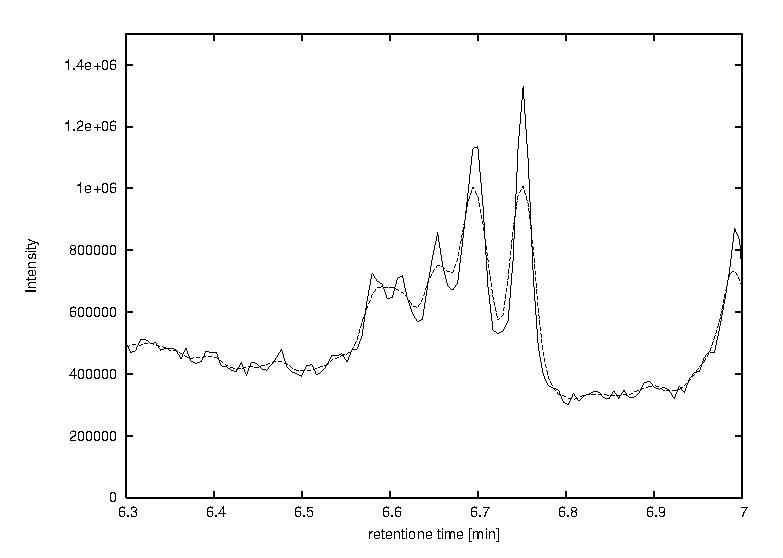
\includegraphics{graphics/pyms-test/tic_mean_smoothed.eps}
\caption{The effect of the 5-point mean moving window average smoothing
on the TIC from 'a0806\_140' data set. The segment 6.3-7.0 minutes is
shown. The original TIC is shown in full line, while the smoothed TIC
is shown in dashed line}
\label{fig:smoothed-mean}
\end{center}
\end{figure}

\begin{figure}[htp]
\begin{center}
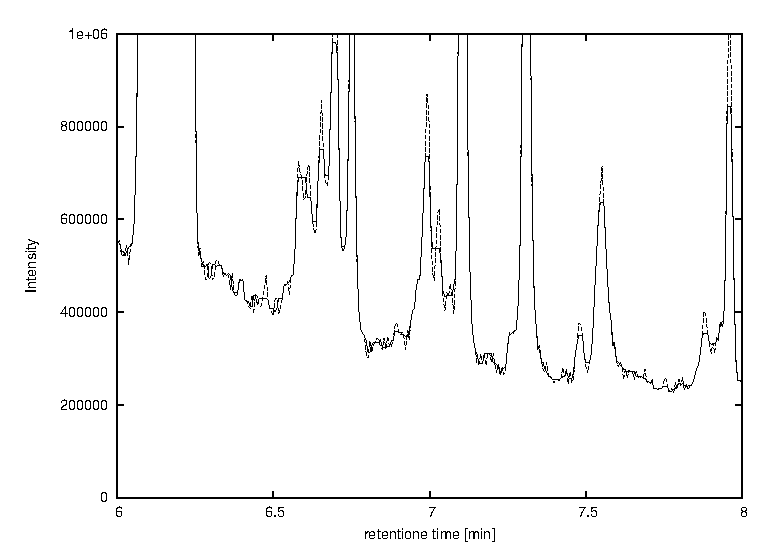
\includegraphics{graphics/pyms-test/tic_median_smoothed.eps}
\caption{The effect of the 5-point median moving window average smoothing
on the TIC from 'a0806\_140' data set. The segment 6.3-7.0 minutes is
shown. The original TIC is shown in full line, while the smoothed TIC
is shown in dashed line}
\label{fig:smoothed-median}
\end{center}
\end{figure}

\section{Time strings}
\label{sec:time-string}

A time string is specification of time interval, that takes the format
'NUMBERs' or 'NUMBERm' for time interval in seconds or minutes. For
example, these are valid time strings: '10s' (10 seconds) and '0.2m'
(0.2 minutes).

\section{\label{sec:baseline_correction}Baseline correction}

\noindent
[ {\em This example is in pyms-test/21} ]

Baseline distortion originating from instrument imperfections and experimental
setup is often observed in mass spectrometry data, and off-line baseline correction
is an important part of data pre-processing. There are many approaches for
baseline correction. One advanced approach is based top-hat transform developed
in mathematical morphology \cite{serra83}, and used extensively in digital image
processing for tasks such as image enhancement.  Top-hat baseline correction was
previously applied in proteomics based mass spectrometry \cite{sauve04}.

PyMS currently implements only top-hat baseline corrector, using the SciPy
package 'ndimage'. For this feature to be available either SciPy (Scientific
Tools for Python \cite{scipy}) must be installed, or the local versions of
scipy's ndimage must be installed. For the SciPy/ndimage installation
instructions please see the section \ref{subsec:scipy-ndmage}.

Application of the top-hat baseline corrector requires the size of the structural
element to be specified. The structural element needs to be larger than the
features one wants to retain in the spectrum after the top-hat transform.
In the example below, the top-hat baseline corrector is applied to the TIC
of the data set 'a0806\_140.CDF', with the structural element of 1.5 minutes:

\begin{verbatim}
from pyms.IO.ANDI.Class import ChemStation
from pyms.Noise.Window import window_smooth
from pyms.Baseline.TopHat import tophat

andi_file = "/home/current/proj/PyMS/pyms-data/a0806_140.CDF"
data = ChemStation(andi_file)

# get the TIC
tic = data.get_tic()

# apply 5-point moving window smoothing & baseline corrector
tic = window_smooth(tic, window=5)
tic_bc = tophat(tic, struct="1.5m")

# save the original and baseline corrected TICs
tic.write("output/tic.dat",minutes=True)
tic_bc.write("output/tic_bc.dat",minutes=True)
\end{verbatim}

\noindent
The original and baseline corrected TICs are saved as files 'tic.dat' and
'tic\_bc.dat', in the directory 'output/'. Running this script produces the
following output:

\begin{verbatim}
$ python proc.py
 -> Processing netCDF file '/home/current/proj/PyMS/pyms-data/a0806_140.CDF'
    [ 3236 scans, masses from 50 to 550 ]
 -> Window smoothing (mean): the wing is 2 point(s)
 -> Top-hat: structural element is 262 point(s)
\end{verbatim}

\noindent
The plot of the original TIC and baseline corrected TIC is shown in
Figure \ref{fig:bc-tophat}.

\begin{figure}[htp]
\begin{center}
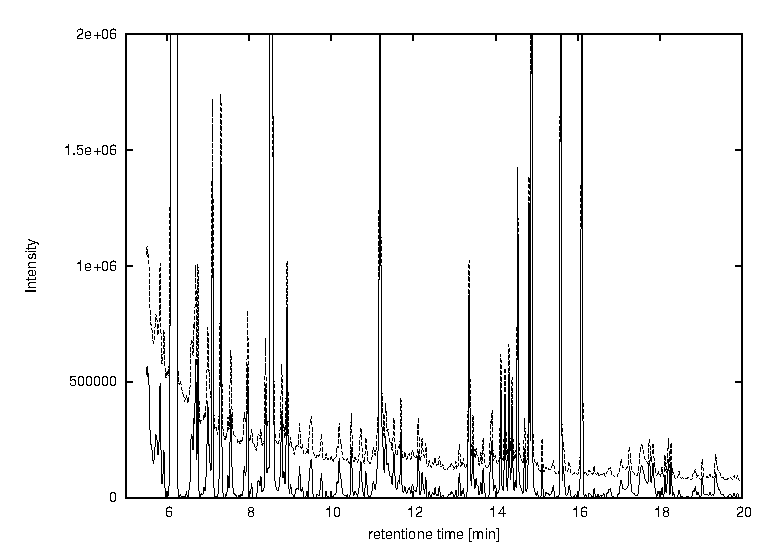
\includegraphics{graphics/pyms-test/tic_bc_tophat.eps}
\caption{The effect of the top-hat baseline corrector with the 1.5 minute
structural element on the TIC for the data 'a0806\_140.CDF'.  The original
TIC is shown in dashed line, while the baseline corrected TIC is shown in
full line.}
\label{fig:bc-tophat}
\end{center}
\end{figure}

It should be noted that top-hat baseline correction can be applied to any
ion chromatogram object (ie. m/z channel ion chromatogram), not only TIC.

